% Mobile-C Library 

%%%%%%%%%%%%%%%%%%%%%%%%%%%%%%%%%%%%%%%%%%%%%%%%%%%%%%%%%%%%%%%%%%%%%%
% Preamble {{{
%\documentclass[11pt]{article}
\documentclass[11pt]{report}
\usepackage{varioref}
\usepackage{times,verbatim,fancyheadings,makeidx}
\usepackage{moreverb}
%\usepackage{psfig}
\usepackage[pdftex]{hyperref}
\usepackage{hypcap}
\usepackage{fullpage}
\usepackage{amssymb,amsmath}
\usepackage{graphicx}
\usepackage{program}
%\headrulewidth 0.0pt
%\hoffset=-0.0625in
%\voffset=0pt
\setlength{\textheight}{9in}
\setlength{\textwidth}{6.5in}
\topmargin=0.05in
\makeindex
% }}} Preamble
%%%%%%%%%%%%%%%%%%%%%%%%%%%%%%%%%%%%%%%%%%%%%%%%%%%%%%%%%%%%%%%%%%%%%%

%%%%%%%%%%%%%%%%%%%%%%%%%%%%%%%%%%%%%%%%%%%%%%%%%%%%%%%%%%%%%%%%%%%%%%
% Title Page {{{
\begin{document}
\thispagestyle{empty}
\begin{center}
%\includegraphics[width=1.8in]{figure/mobilec_logo.png}


\vspace{0.5in}
{\Huge\sf\bf User's Guide for Programming iMobot} \\
\vspace{2.0in}
{\large\sf\bf\today}
%September 20, 2007
\end{center}

\pagebreak
% }}} Title Page
%%%%%%%%%%%%%%%%%%%%%%%%%%%%%%%%%%%%%%%%%%%%%%%%%%%%%%%%%%%%%%%%%%%%%%

%%%%%%%%%%%%%%%%%%%%%%%%%%%%%%%%%%%%%%%%%%%%%%%%%%%%%%%%%%%%%%%%%%%%%%
% Abstract {{{
%\phantomsection
%\addcontentsline{toc}{chapter}{Abstract}
\begin{abstract} 
This user's guide describes how to control an iMobot robotic module.

\end{abstract}
\pagebreak
% Abstract }}}
%%%%%%%%%%%%%%%%%%%%%%%%%%%%%%%%%%%%%%%%%%%%%%%%%%%%%%%%%%%%%%%%%%%%%%

%%%%%%%%%%%%%%%%%%%%%%%%%%%%%%%%%%%%%%%%%%%%%%%%%%%%%%%%%%%%%%%%%%%%%%
% Table of Contents {{{
\pagenumbering{roman}
\setcounter{page}{1}
\tableofcontents
\pagebreak
% }}} Table of Contents
%%%%%%%%%%%%%%%%%%%%%%%%%%%%%%%%%%%%%%%%%%%%%%%%%%%%%%%%%%%%%%%%%%%%%%

%%%%%%%%%%%%%%%%%%%%%%%%%%%%%%%%%%%%%%%%%%%%%%%%%%%%%%%%%%%%%%%%%%%%%%
% Part 1 {{{
\pagenumbering{arabic}
\setcounter{page}{1}
\pagebreak
% }}} Part 1 
%%%%%%%%%%%%%%%%%%%%%%%%%%%%%%%%%%%%%%%%%%%%%%%%%%%%%%%%%%%%%%%%%%%%%%

%%%%%%%%%%%%%%%%%%%%%%%%%%%%%%%%%%%%%%%%%%%%%%%%%%%%%%%%%%%%%%%%%%%%%%
% Introduction {{{
%\pagenumbering{arabic}
%\setcounter{page}{1}
%\pagestyle{fancy}
%\chapter{Introduction}
%\pagebreak
% }}} Introduction
%%%%%%%%%%%%%%%%%%%%%%%%%%%%%%%%%%%%%%%%%%%%%%%%%%%%%%%%%%%%%%%%%%%%%%

\chapter{Getting Started}
This short guide will enable you to run the provided demo program,
``simple.cpp'', on the iMobot.
\begin{enumerate}
\item Download and install a VNC client
  \begin{itemize}
  \item For Windows, you may download and install TightVNC from \texttt{http://www.tightvnc.com}.
  \item For Mac OS X, you may download and install Chicken of the VNC from\\
  \texttt{http://sourceforge.net/projects/cotvnc/}
  \end{itemize}
\item Log in to the imobot with a VNC client. 
\item Connect to the iMobot with your VNC client. The default address of the iMobot is \texttt{192.168.0.123}.
\item Open and execute the demo program.
  \begin{enumerate}
  \item Copy the demo program to your home directory with the command\\
  \texttt{cp /usr/local/ch/package/chimobot/demos/simple.cpp \textasciitilde/}
  \item Open the demo program with ChIDE. You may left click on the desktop to open the menu, and select \texttt{Applications -> Accessories -> ChIDE}.
  \item Click on \texttt{File -> Open} within ChIDE and open the program, \texttt{simple.cpp}. 
  \item Click on the ``Run'' button, located near the top right of the ChIDE Window. The robot should now run the program.
  \end{enumerate}
\end{enumerate}

\chapter{Graphical Control Interface}
\begin{figure}
\begin{center}
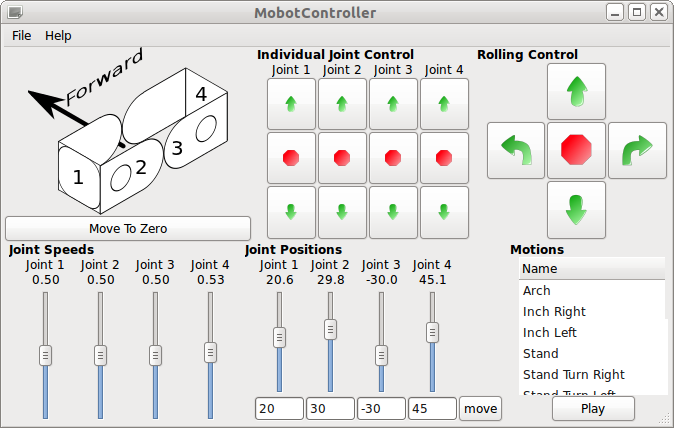
\includegraphics[width=4in]{gui_screenshot.png}
\caption{\label{fig:gui}The iMobot Graphical Control Interface.}
\end{center}
\end{figure}
The iMobot comes with a graphical control interface for controlling the iMobot.
The control interface is able to perform simple locomotion tasks, and can be
used to determine the joint angles of the iMobot. A screenshot of the interface
is shown in Figure \ref{fig:gui}.

The graphical interface can be found in the application menu of the iMobot. Once
a VNC connection to the iMobot has been established, simply left click on the
desktop to bring up the menu, and select the item \texttt{Applications ->
Accessories -> iMobot Controller}. Once the controller starts, it needs to be
initialized in order to establish communication with the motor controllers.
This is done by clicking on \texttt{File -> Init Local I2C Bus}. Ensure that 
the application is connected by ensuring that the status bar at the bottom of the
application displays ``Connected''. 

The graphical interface is composed of four basic components, as shown in
Figure \ref{fig:gui}. The first section, labeled with the red ``1'',
is a section of four sliders. Each slider controls the motor speed of a joint.

The next section, labeled ``2'', are controls which can be used to move each
joint independantly. The upward arrows indicate forward rotation, the stop
buttons stop the motors, and the downward arrows indicate backward motion.
Below the downward arrows are textboxes which display the current angle of each
joint.

The next section, labeled ``3'', contain buttons used for moving the iMobot. 
The arrows indicate forwards and backwards motion, along with turning and
sideways inchworming motions. The large stop sign button stops all motions
on the iMobot. The button labeled ``Home'' causes the iMobot to move all joints
back to their home position. 

The final section, labeled ``4'', contain preprogramed gaits for the iMobot.
To execute a gait, simply select the desired gait by left-clicking on its name,
and click the ``Play'' button.

%%%%%%%%%%%%%%%%%%%%%%%%%%%%%%%%%%%%%%%%%%%%%%%%%%%%%%%%%%%%%%%%%%%%%%
% SUB: Overview of Sample Application Programs {{{
\chapter{Overview of a Sample Application Program}
The following program is a simple program which moves some joints on the iMobot
before initializing the robot to listen for incoming Bluetooth commands.
\subsection{simple.cpp \label{subsec:simple.cpp}}
\listinginput{1}{../Demos/simple_cpp/simple.cpp}
\subsection{Explanation of simple.cpp}
\begin{itemize}
\item Lines 1-3 include the chimobot Ch package. These lines are necessary for
running Ch programs which control the iMobot. 
\item Lines 8-10 declare some local variables that are used throughout the program.
\item Line 10 declares the \texttt{robot} object, which represents the
capabilities of the iMobot module. This object contains various member
functions which may be executed by the user.
\item Lines 13-16 send commands to the iMobot to move all the joints to their
zero position.
\item Line 17 causes the program to wait until all the joints have stopped moving. 
\item Lines 20 and 21 instruct the robot to rotate joints 2 and 3 to rotate 90
degrees. Note that the joint numbers start at 0, so joints 2 and 3 are the
third and fourth joints, respectively. 
\item Lines 23 and 24 cause the program to wait until the third and fourth
joints have stopped moving.
\item Lines 26 and 27 instruct the robot to turn the third and fourth joints
back to their original zero position.
\item Lines 28 and 29 cause the program to wait until the third and fourth
joints have stopped moving.
\item Lines 33 and 34 start the Bluetooth listening service on channel 20,
which listens for Bluetooth remote commands and controls the robot accordingly. 
\item Line 37 terminates the robot control.
\end{itemize}

%%%%%%%%%%%%%%%%%%%%%%%%%%%%%%%%%%%%%%%%%%%%%%%%%%%%%%%%%%%%%%%%%%%%%%
% SUB: Execution of Sample Applications {{{
%\section{Execution of Sample Applications}
%%%%%%%%%%%%%%%%%%%%%%%%%%%%%%%%%%%%%%%%%%%%%%%%%%%%%%%%%%%%%%%%%%%%%%
% Appendix {{{
\appendix
\chapter{iMobot API}
% Mobile-C Library 

%%%%%%%%%%%%%%%%%%%%%%%%%%%%%%%%%%%%%%%%%%%%%%%%%%%%%%%%%%%%%%%%%%%%%%
% Preamble {{{
%\documentclass[11pt]{article}
\documentclass[11pt]{report}
\usepackage{varioref}
\usepackage{times,verbatim,fancyheadings,makeidx}
\usepackage{moreverb}
%\usepackage{psfig}
\usepackage[pdftex]{hyperref}
\usepackage{hypcap}
\usepackage{fullpage}
\usepackage{amssymb,amsmath}
\usepackage{graphicx}
\usepackage{program}
%\headrulewidth 0.0pt
%\hoffset=-0.0625in
%\voffset=0pt
\setlength{\textheight}{9in}
\setlength{\textwidth}{6.5in}
\topmargin=0.05in
\makeindex
% }}} Preamble
%%%%%%%%%%%%%%%%%%%%%%%%%%%%%%%%%%%%%%%%%%%%%%%%%%%%%%%%%%%%%%%%%%%%%%

%%%%%%%%%%%%%%%%%%%%%%%%%%%%%%%%%%%%%%%%%%%%%%%%%%%%%%%%%%%%%%%%%%%%%%
% Title Page {{{
\begin{document}
\thispagestyle{empty}
\begin{center}
%\includegraphics[width=1.8in]{figure/mobilec_logo.png}


\vspace{0.5in}
{\Huge\sf\bf User's Guide for Programming iMobot} \\
\vspace{2.0in}
{\large\sf\bf\today}
%September 20, 2007
\end{center}

\pagebreak
% }}} Title Page
%%%%%%%%%%%%%%%%%%%%%%%%%%%%%%%%%%%%%%%%%%%%%%%%%%%%%%%%%%%%%%%%%%%%%%

%%%%%%%%%%%%%%%%%%%%%%%%%%%%%%%%%%%%%%%%%%%%%%%%%%%%%%%%%%%%%%%%%%%%%%
% Abstract {{{
%\phantomsection
%\addcontentsline{toc}{chapter}{Abstract}
\begin{abstract} 
This library implements control functions for controlling an iMobot
robotic module.

\end{abstract}
\pagebreak
% Abstract }}}
%%%%%%%%%%%%%%%%%%%%%%%%%%%%%%%%%%%%%%%%%%%%%%%%%%%%%%%%%%%%%%%%%%%%%%

%%%%%%%%%%%%%%%%%%%%%%%%%%%%%%%%%%%%%%%%%%%%%%%%%%%%%%%%%%%%%%%%%%%%%%
% Table of Contents {{{
\pagenumbering{roman}
\setcounter{page}{1}
\tableofcontents
\pagebreak
% }}} Table of Contents
%%%%%%%%%%%%%%%%%%%%%%%%%%%%%%%%%%%%%%%%%%%%%%%%%%%%%%%%%%%%%%%%%%%%%%

%%%%%%%%%%%%%%%%%%%%%%%%%%%%%%%%%%%%%%%%%%%%%%%%%%%%%%%%%%%%%%%%%%%%%%
% Part 1 {{{
\pagenumbering{arabic}
\setcounter{page}{1}
\pagebreak
% }}} Part 1 
%%%%%%%%%%%%%%%%%%%%%%%%%%%%%%%%%%%%%%%%%%%%%%%%%%%%%%%%%%%%%%%%%%%%%%

%%%%%%%%%%%%%%%%%%%%%%%%%%%%%%%%%%%%%%%%%%%%%%%%%%%%%%%%%%%%%%%%%%%%%%
% Introduction {{{
%\pagenumbering{arabic}
%\setcounter{page}{1}
%\pagestyle{fancy}
%\chapter{Introduction}
%\pagebreak
% }}} Introduction
%%%%%%%%%%%%%%%%%%%%%%%%%%%%%%%%%%%%%%%%%%%%%%%%%%%%%%%%%%%%%%%%%%%%%%

\chapter{Getting Started}
This short guide will enable you to run the provided demo program,
``simple.cpp'', on the iMobot.
\begin{enumerate}
\item Log in to the imobot. In order to do this, you will need a VNC client. 
  \begin{itemize}
  \item For Windows, you may download and install TightVNC from \texttt{http://www.tightvnc.com}.
  \item For Mac OS X, you may download and install Chicken of the VNC from \texttt{http://sourceforge.net/projects/cotvnc/}.
  \end{itemize}
\item Connect to the iMobot with your VNC client. The default address of the iMobot is \texttt{192.168.0.123}.
\item Copy the demo program to your home directory with the command ``\texttt{cp /usr/local/ch/package/chimobot/demos/simple.cpp ~/}''.
\item Open the demo program with ChIDE. You may left click on the desktop to open the menu, and select \texttt{Applications -> Accessories -> ChIDE}.
\item Click on \texttt{File -> Open} within ChIDE and open the program, \texttt{simple.cpp}. 
\item Click on the ``Run'' button, located near the top right of the ChIDE Window. The robot should now run the program.
\end{enumerate}

\chapter{Gtk iMobot Controller Guide}
\begin{figure}
\begin{center}
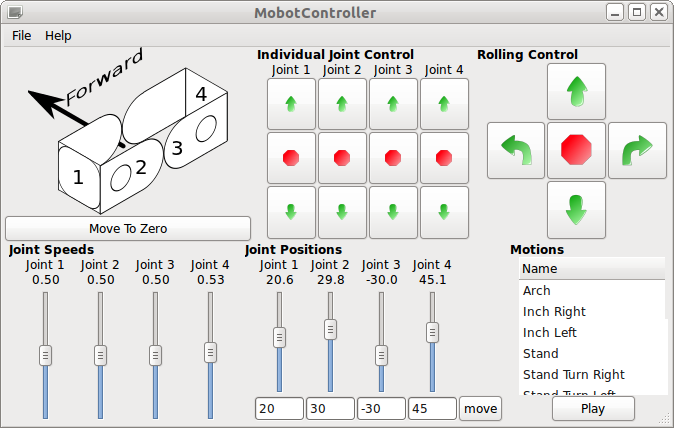
\includegraphics[width=4in]{gui_screenshot.png}
\caption{\label{fig:gui}The iMobot Graphical Control Interface.}
\end{center}
\end{figure}
The iMobot comes with a graphical control interface for controlling the iMobot.
The control interface is able to perform simple locomotion tasks, and can be
used to determine the joint angles of the iMobot. A screenshot of the interface
is shown in Figure \ref{fig:gui}.

The graphical interface can be found in the application menu of the iMobot. Once
a VNC connection to the iMobot has been established, simply left click on the
desktop to bring up the menu, and select the item \texttt{Applications ->
Accessories -> iMobot Controller}. Once the controller starts, it needs to be
initialized in order to establish communication with the motor controllers.
This is done by clicking on \texttt{File -> Init Local I2C Bus}. Ensure that 
the application is connected by ensuring that the status bar at the bottom of the
application displays ``Connected''. 

The graphical interface is composed of four basic components, as shown in
Figure \ref{fig:gui}. The first section, labeled with the red ``1'',
is a section of four sliders. Each slider controls the motor speed of a joint.

The next section, labeled ``2'', are controls which can be used to move each
joint independantly. The upward arrows indicate forward rotation, the stop
buttons stop the motors, and the downward arrows indicate backward motion.
Below the downward arrows are textboxes which display the current angle of each
joint.

The next section, labeled ``3'', contain buttons used for moving the iMobot. 
The arrows indicate forwards and backwards motion, along with turning and
sideways inchworming motions. The large stop sign button stops all motions
on the iMobot. The button labeled ``Home'' causes the iMobot to move all joints
back to their home position. 

The final section, labeled ``4'', contain preprogramed gaits for the iMobot.
To execute a gait, simply select the desired gait by left-clicking on its name,
and click the ``Play'' button.

%%%%%%%%%%%%%%%%%%%%%%%%%%%%%%%%%%%%%%%%%%%%%%%%%%%%%%%%%%%%%%%%%%%%%%
% SUB: Overview of Sample Application Programs {{{
\chapter{Overview of a Sample Application Program}
The following program is a simple program which moves some joints on the iMobot
before initializing the robot to listen for incoming Bluetooth commands.
\subsection{simple.cpp \label{subsec:simple.cpp}}
\listinginput{1}{../Demos/simple_cpp/simple.cpp}
\subsection{Explanation of simple.cpp}
\begin{itemize}
\item Lines 1-3 include the chimobot Ch package. These lines are necessary for
running Ch programs which control the iMobot. 
\item Lines 8-10 declare some local variables that are used throughout the program.
\item Line 10 declares the \texttt{robot} object, which represents the
capabilities of the iMobot module. This object contains various member
functions which may be executed by the user.
\item Lines 13-16 send commands to the iMobot to move all the joints to their
zero position.
\item Line 17 causes the program to wait until all the joints have stopped moving. 
\item Lines 20 and 21 instruct the robot to rotate joints 2 and 3 to rotate 90
degrees. Note that the joint numbers start at 0, so joints 2 and 3 are the
third and fourth joints, respectively. 
\item Lines 23 and 24 cause the program to wait until the third and fourth
joints have stopped moving.
\item Lines 26 and 27 instruct the robot to turn the third and fourth joints
back to their original zero position.
\item Lines 28 and 29 cause the program to wait until the third and fourth
joints have stopped moving.
\item Lines 33 and 34 start the Bluetooth listening service on channel 20,
which listens for Bluetooth remote commands and controls the robot accordingly. 
\item Line 37 terminates the robot control.
\end{itemize}

%%%%%%%%%%%%%%%%%%%%%%%%%%%%%%%%%%%%%%%%%%%%%%%%%%%%%%%%%%%%%%%%%%%%%%
% SUB: Execution of Sample Applications {{{
%\section{Execution of Sample Applications}
%%%%%%%%%%%%%%%%%%%%%%%%%%%%%%%%%%%%%%%%%%%%%%%%%%%%%%%%%%%%%%%%%%%%%%
% Appendix {{{
\appendix
\chapter{libimobot API}
% Mobile-C Library 

%%%%%%%%%%%%%%%%%%%%%%%%%%%%%%%%%%%%%%%%%%%%%%%%%%%%%%%%%%%%%%%%%%%%%%
% Preamble {{{
%\documentclass[11pt]{article}
\documentclass[11pt]{report}
\usepackage{varioref}
\usepackage{times,verbatim,fancyheadings,makeidx}
\usepackage{moreverb}
%\usepackage{psfig}
\usepackage[pdftex]{hyperref}
\usepackage{hypcap}
\usepackage{fullpage}
\usepackage{amssymb,amsmath}
\usepackage{graphicx}
\usepackage{program}
%\headrulewidth 0.0pt
%\hoffset=-0.0625in
%\voffset=0pt
\setlength{\textheight}{9in}
\setlength{\textwidth}{6.5in}
\topmargin=0.05in
\makeindex
% }}} Preamble
%%%%%%%%%%%%%%%%%%%%%%%%%%%%%%%%%%%%%%%%%%%%%%%%%%%%%%%%%%%%%%%%%%%%%%

%%%%%%%%%%%%%%%%%%%%%%%%%%%%%%%%%%%%%%%%%%%%%%%%%%%%%%%%%%%%%%%%%%%%%%
% Title Page {{{
\begin{document}
\thispagestyle{empty}
\begin{center}
%\includegraphics[width=1.8in]{figure/mobilec_logo.png}


\vspace{0.5in}
{\Huge\sf\bf User's Guide for Programming iMobot} \\
\vspace{2.0in}
{\large\sf\bf\today}
%September 20, 2007
\end{center}

\pagebreak
% }}} Title Page
%%%%%%%%%%%%%%%%%%%%%%%%%%%%%%%%%%%%%%%%%%%%%%%%%%%%%%%%%%%%%%%%%%%%%%

%%%%%%%%%%%%%%%%%%%%%%%%%%%%%%%%%%%%%%%%%%%%%%%%%%%%%%%%%%%%%%%%%%%%%%
% Abstract {{{
%\phantomsection
%\addcontentsline{toc}{chapter}{Abstract}
\begin{abstract} 
This library implements control functions for controlling an iMobot
robotic module.

\end{abstract}
\pagebreak
% Abstract }}}
%%%%%%%%%%%%%%%%%%%%%%%%%%%%%%%%%%%%%%%%%%%%%%%%%%%%%%%%%%%%%%%%%%%%%%

%%%%%%%%%%%%%%%%%%%%%%%%%%%%%%%%%%%%%%%%%%%%%%%%%%%%%%%%%%%%%%%%%%%%%%
% Table of Contents {{{
\pagenumbering{roman}
\setcounter{page}{1}
\tableofcontents
\pagebreak
% }}} Table of Contents
%%%%%%%%%%%%%%%%%%%%%%%%%%%%%%%%%%%%%%%%%%%%%%%%%%%%%%%%%%%%%%%%%%%%%%

%%%%%%%%%%%%%%%%%%%%%%%%%%%%%%%%%%%%%%%%%%%%%%%%%%%%%%%%%%%%%%%%%%%%%%
% Part 1 {{{
\pagenumbering{arabic}
\setcounter{page}{1}
\pagebreak
% }}} Part 1 
%%%%%%%%%%%%%%%%%%%%%%%%%%%%%%%%%%%%%%%%%%%%%%%%%%%%%%%%%%%%%%%%%%%%%%

%%%%%%%%%%%%%%%%%%%%%%%%%%%%%%%%%%%%%%%%%%%%%%%%%%%%%%%%%%%%%%%%%%%%%%
% Introduction {{{
%\pagenumbering{arabic}
%\setcounter{page}{1}
%\pagestyle{fancy}
%\chapter{Introduction}
%\pagebreak
% }}} Introduction
%%%%%%%%%%%%%%%%%%%%%%%%%%%%%%%%%%%%%%%%%%%%%%%%%%%%%%%%%%%%%%%%%%%%%%

\chapter{Getting Started}
This short guide will enable you to run the provided demo program,
``simple.cpp'', on the iMobot.
\begin{enumerate}
\item Log in to the imobot. In order to do this, you will need a VNC client. 
  \begin{itemize}
  \item For Windows, you may download and install TightVNC from \texttt{http://www.tightvnc.com}.
  \item For Mac OS X, you may download and install Chicken of the VNC from \texttt{http://sourceforge.net/projects/cotvnc/}.
  \end{itemize}
\item Connect to the iMobot with your VNC client. The default address of the iMobot is \texttt{192.168.0.123}.
\item Copy the demo program to your home directory with the command ``\texttt{cp /usr/local/ch/package/chimobot/demos/simple.cpp ~/}''.
\item Open the demo program with ChIDE. You may left click on the desktop to open the menu, and select \texttt{Applications -> Accessories -> ChIDE}.
\item Click on \texttt{File -> Open} within ChIDE and open the program, \texttt{simple.cpp}. 
\item Click on the ``Run'' button, located near the top right of the ChIDE Window. The robot should now run the program.
\end{enumerate}

\chapter{Gtk iMobot Controller Guide}
\begin{figure}
\begin{center}
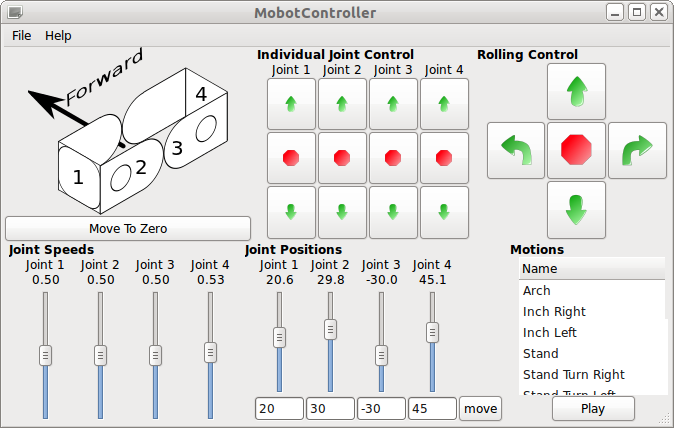
\includegraphics[width=4in]{gui_screenshot.png}
\caption{\label{fig:gui}The iMobot Graphical Control Interface.}
\end{center}
\end{figure}
The iMobot comes with a graphical control interface for controlling the iMobot.
The control interface is able to perform simple locomotion tasks, and can be
used to determine the joint angles of the iMobot. A screenshot of the interface
is shown in Figure \ref{fig:gui}.

The graphical interface can be found in the application menu of the iMobot. Once
a VNC connection to the iMobot has been established, simply left click on the
desktop to bring up the menu, and select the item \texttt{Applications ->
Accessories -> iMobot Controller}. Once the controller starts, it needs to be
initialized in order to establish communication with the motor controllers.
This is done by clicking on \texttt{File -> Init Local I2C Bus}. Ensure that 
the application is connected by ensuring that the status bar at the bottom of the
application displays ``Connected''. 

The graphical interface is composed of four basic components, as shown in
Figure \ref{fig:gui}. The first section, labeled with the red ``1'',
is a section of four sliders. Each slider controls the motor speed of a joint.

The next section, labeled ``2'', are controls which can be used to move each
joint independantly. The upward arrows indicate forward rotation, the stop
buttons stop the motors, and the downward arrows indicate backward motion.
Below the downward arrows are textboxes which display the current angle of each
joint.

The next section, labeled ``3'', contain buttons used for moving the iMobot. 
The arrows indicate forwards and backwards motion, along with turning and
sideways inchworming motions. The large stop sign button stops all motions
on the iMobot. The button labeled ``Home'' causes the iMobot to move all joints
back to their home position. 

The final section, labeled ``4'', contain preprogramed gaits for the iMobot.
To execute a gait, simply select the desired gait by left-clicking on its name,
and click the ``Play'' button.

%%%%%%%%%%%%%%%%%%%%%%%%%%%%%%%%%%%%%%%%%%%%%%%%%%%%%%%%%%%%%%%%%%%%%%
% SUB: Overview of Sample Application Programs {{{
\chapter{Overview of a Sample Application Program}
The following program is a simple program which moves some joints on the iMobot
before initializing the robot to listen for incoming Bluetooth commands.
\subsection{simple.cpp \label{subsec:simple.cpp}}
\listinginput{1}{../Demos/simple_cpp/simple.cpp}
\subsection{Explanation of simple.cpp}
\begin{itemize}
\item Lines 1-3 include the chimobot Ch package. These lines are necessary for
running Ch programs which control the iMobot. 
\item Lines 8-10 declare some local variables that are used throughout the program.
\item Line 10 declares the \texttt{robot} object, which represents the
capabilities of the iMobot module. This object contains various member
functions which may be executed by the user.
\item Lines 13-16 send commands to the iMobot to move all the joints to their
zero position.
\item Line 17 causes the program to wait until all the joints have stopped moving. 
\item Lines 20 and 21 instruct the robot to rotate joints 2 and 3 to rotate 90
degrees. Note that the joint numbers start at 0, so joints 2 and 3 are the
third and fourth joints, respectively. 
\item Lines 23 and 24 cause the program to wait until the third and fourth
joints have stopped moving.
\item Lines 26 and 27 instruct the robot to turn the third and fourth joints
back to their original zero position.
\item Lines 28 and 29 cause the program to wait until the third and fourth
joints have stopped moving.
\item Lines 33 and 34 start the Bluetooth listening service on channel 20,
which listens for Bluetooth remote commands and controls the robot accordingly. 
\item Line 37 terminates the robot control.
\end{itemize}

%%%%%%%%%%%%%%%%%%%%%%%%%%%%%%%%%%%%%%%%%%%%%%%%%%%%%%%%%%%%%%%%%%%%%%
% SUB: Execution of Sample Applications {{{
%\section{Execution of Sample Applications}
%%%%%%%%%%%%%%%%%%%%%%%%%%%%%%%%%%%%%%%%%%%%%%%%%%%%%%%%%%%%%%%%%%%%%%
% Appendix {{{
\appendix
\chapter{libimobot API}
% Mobile-C Library 

%%%%%%%%%%%%%%%%%%%%%%%%%%%%%%%%%%%%%%%%%%%%%%%%%%%%%%%%%%%%%%%%%%%%%%
% Preamble {{{
%\documentclass[11pt]{article}
\documentclass[11pt]{report}
\usepackage{varioref}
\usepackage{times,verbatim,fancyheadings,makeidx}
\usepackage{moreverb}
%\usepackage{psfig}
\usepackage[pdftex]{hyperref}
\usepackage{hypcap}
\usepackage{fullpage}
\usepackage{amssymb,amsmath}
\usepackage{graphicx}
\usepackage{program}
%\headrulewidth 0.0pt
%\hoffset=-0.0625in
%\voffset=0pt
\setlength{\textheight}{9in}
\setlength{\textwidth}{6.5in}
\topmargin=0.05in
\makeindex
% }}} Preamble
%%%%%%%%%%%%%%%%%%%%%%%%%%%%%%%%%%%%%%%%%%%%%%%%%%%%%%%%%%%%%%%%%%%%%%

%%%%%%%%%%%%%%%%%%%%%%%%%%%%%%%%%%%%%%%%%%%%%%%%%%%%%%%%%%%%%%%%%%%%%%
% Title Page {{{
\begin{document}
\thispagestyle{empty}
\begin{center}
%\includegraphics[width=1.8in]{figure/mobilec_logo.png}


\vspace{0.5in}
{\Huge\sf\bf User's Guide for Programming iMobot} \\
\vspace{2.0in}
{\large\sf\bf\today}
%September 20, 2007
\end{center}

\pagebreak
% }}} Title Page
%%%%%%%%%%%%%%%%%%%%%%%%%%%%%%%%%%%%%%%%%%%%%%%%%%%%%%%%%%%%%%%%%%%%%%

%%%%%%%%%%%%%%%%%%%%%%%%%%%%%%%%%%%%%%%%%%%%%%%%%%%%%%%%%%%%%%%%%%%%%%
% Abstract {{{
%\phantomsection
%\addcontentsline{toc}{chapter}{Abstract}
\begin{abstract} 
This library implements control functions for controlling an iMobot
robotic module.

\end{abstract}
\pagebreak
% Abstract }}}
%%%%%%%%%%%%%%%%%%%%%%%%%%%%%%%%%%%%%%%%%%%%%%%%%%%%%%%%%%%%%%%%%%%%%%

%%%%%%%%%%%%%%%%%%%%%%%%%%%%%%%%%%%%%%%%%%%%%%%%%%%%%%%%%%%%%%%%%%%%%%
% Table of Contents {{{
\pagenumbering{roman}
\setcounter{page}{1}
\tableofcontents
\pagebreak
% }}} Table of Contents
%%%%%%%%%%%%%%%%%%%%%%%%%%%%%%%%%%%%%%%%%%%%%%%%%%%%%%%%%%%%%%%%%%%%%%

%%%%%%%%%%%%%%%%%%%%%%%%%%%%%%%%%%%%%%%%%%%%%%%%%%%%%%%%%%%%%%%%%%%%%%
% Part 1 {{{
\pagenumbering{arabic}
\setcounter{page}{1}
\pagebreak
% }}} Part 1 
%%%%%%%%%%%%%%%%%%%%%%%%%%%%%%%%%%%%%%%%%%%%%%%%%%%%%%%%%%%%%%%%%%%%%%

%%%%%%%%%%%%%%%%%%%%%%%%%%%%%%%%%%%%%%%%%%%%%%%%%%%%%%%%%%%%%%%%%%%%%%
% Introduction {{{
%\pagenumbering{arabic}
%\setcounter{page}{1}
%\pagestyle{fancy}
%\chapter{Introduction}
%\pagebreak
% }}} Introduction
%%%%%%%%%%%%%%%%%%%%%%%%%%%%%%%%%%%%%%%%%%%%%%%%%%%%%%%%%%%%%%%%%%%%%%

\chapter{Getting Started}
This short guide will enable you to run the provided demo program,
``simple.cpp'', on the iMobot.
\begin{enumerate}
\item Log in to the imobot. In order to do this, you will need a VNC client. 
  \begin{itemize}
  \item For Windows, you may download and install TightVNC from \texttt{http://www.tightvnc.com}.
  \item For Mac OS X, you may download and install Chicken of the VNC from \texttt{http://sourceforge.net/projects/cotvnc/}.
  \end{itemize}
\item Connect to the iMobot with your VNC client. The default address of the iMobot is \texttt{192.168.0.123}.
\item Copy the demo program to your home directory with the command ``\texttt{cp /usr/local/ch/package/chimobot/demos/simple.cpp ~/}''.
\item Open the demo program with ChIDE. You may left click on the desktop to open the menu, and select \texttt{Applications -> Accessories -> ChIDE}.
\item Click on \texttt{File -> Open} within ChIDE and open the program, \texttt{simple.cpp}. 
\item Click on the ``Run'' button, located near the top right of the ChIDE Window. The robot should now run the program.
\end{enumerate}

\chapter{Gtk iMobot Controller Guide}
\begin{figure}
\begin{center}
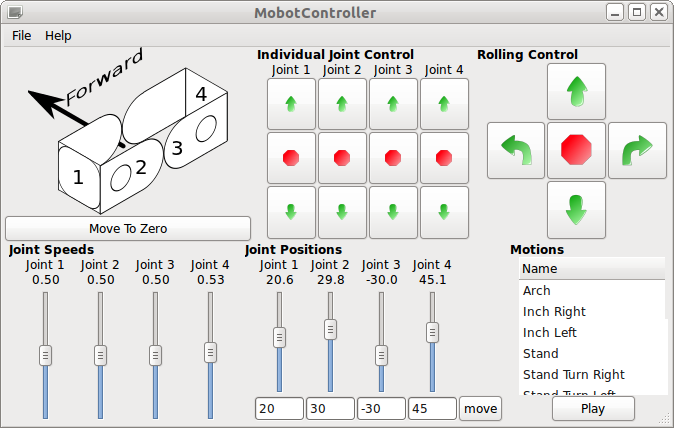
\includegraphics[width=4in]{gui_screenshot.png}
\caption{\label{fig:gui}The iMobot Graphical Control Interface.}
\end{center}
\end{figure}
The iMobot comes with a graphical control interface for controlling the iMobot.
The control interface is able to perform simple locomotion tasks, and can be
used to determine the joint angles of the iMobot. A screenshot of the interface
is shown in Figure \ref{fig:gui}.

The graphical interface can be found in the application menu of the iMobot. Once
a VNC connection to the iMobot has been established, simply left click on the
desktop to bring up the menu, and select the item \texttt{Applications ->
Accessories -> iMobot Controller}. Once the controller starts, it needs to be
initialized in order to establish communication with the motor controllers.
This is done by clicking on \texttt{File -> Init Local I2C Bus}. Ensure that 
the application is connected by ensuring that the status bar at the bottom of the
application displays ``Connected''. 

The graphical interface is composed of four basic components, as shown in
Figure \ref{fig:gui}. The first section, labeled with the red ``1'',
is a section of four sliders. Each slider controls the motor speed of a joint.

The next section, labeled ``2'', are controls which can be used to move each
joint independantly. The upward arrows indicate forward rotation, the stop
buttons stop the motors, and the downward arrows indicate backward motion.
Below the downward arrows are textboxes which display the current angle of each
joint.

The next section, labeled ``3'', contain buttons used for moving the iMobot. 
The arrows indicate forwards and backwards motion, along with turning and
sideways inchworming motions. The large stop sign button stops all motions
on the iMobot. The button labeled ``Home'' causes the iMobot to move all joints
back to their home position. 

The final section, labeled ``4'', contain preprogramed gaits for the iMobot.
To execute a gait, simply select the desired gait by left-clicking on its name,
and click the ``Play'' button.

%%%%%%%%%%%%%%%%%%%%%%%%%%%%%%%%%%%%%%%%%%%%%%%%%%%%%%%%%%%%%%%%%%%%%%
% SUB: Overview of Sample Application Programs {{{
\chapter{Overview of a Sample Application Program}
The following program is a simple program which moves some joints on the iMobot
before initializing the robot to listen for incoming Bluetooth commands.
\subsection{simple.cpp \label{subsec:simple.cpp}}
\listinginput{1}{../Demos/simple_cpp/simple.cpp}
\subsection{Explanation of simple.cpp}
\begin{itemize}
\item Lines 1-3 include the chimobot Ch package. These lines are necessary for
running Ch programs which control the iMobot. 
\item Lines 8-10 declare some local variables that are used throughout the program.
\item Line 10 declares the \texttt{robot} object, which represents the
capabilities of the iMobot module. This object contains various member
functions which may be executed by the user.
\item Lines 13-16 send commands to the iMobot to move all the joints to their
zero position.
\item Line 17 causes the program to wait until all the joints have stopped moving. 
\item Lines 20 and 21 instruct the robot to rotate joints 2 and 3 to rotate 90
degrees. Note that the joint numbers start at 0, so joints 2 and 3 are the
third and fourth joints, respectively. 
\item Lines 23 and 24 cause the program to wait until the third and fourth
joints have stopped moving.
\item Lines 26 and 27 instruct the robot to turn the third and fourth joints
back to their original zero position.
\item Lines 28 and 29 cause the program to wait until the third and fourth
joints have stopped moving.
\item Lines 33 and 34 start the Bluetooth listening service on channel 20,
which listens for Bluetooth remote commands and controls the robot accordingly. 
\item Line 37 terminates the robot control.
\end{itemize}

%%%%%%%%%%%%%%%%%%%%%%%%%%%%%%%%%%%%%%%%%%%%%%%%%%%%%%%%%%%%%%%%%%%%%%
% SUB: Execution of Sample Applications {{{
%\section{Execution of Sample Applications}
%%%%%%%%%%%%%%%%%%%%%%%%%%%%%%%%%%%%%%%%%%%%%%%%%%%%%%%%%%%%%%%%%%%%%%
% Appendix {{{
\appendix
\chapter{libimobot API}
\input{api/libimobot}
\pagebreak
% }}} Appendix 
%%%%%%%%%%%%%%%%%%%%%%%%%%%%%%%%%%%%%%%%%%%%%%%%%%%%%%%%%%%%%%%%%%%%%%

%%%%%%%%%%%%%%%%%%%%%%%%%%%%%%%%%%%%%%%%%%%%%%%%%%%%%%%%%%%%%%%%%%%%%%
% Index {{{
\phantomsection
\addcontentsline{toc}{chapter}{Index}
\printindex
% }}} Index 
%%%%%%%%%%%%%%%%%%%%%%%%%%%%%%%%%%%%%%%%%%%%%%%%%%%%%%%%%%%%%%%%%%%%%%
\end{document}

\pagebreak
% }}} Appendix 
%%%%%%%%%%%%%%%%%%%%%%%%%%%%%%%%%%%%%%%%%%%%%%%%%%%%%%%%%%%%%%%%%%%%%%

%%%%%%%%%%%%%%%%%%%%%%%%%%%%%%%%%%%%%%%%%%%%%%%%%%%%%%%%%%%%%%%%%%%%%%
% Index {{{
\phantomsection
\addcontentsline{toc}{chapter}{Index}
\printindex
% }}} Index 
%%%%%%%%%%%%%%%%%%%%%%%%%%%%%%%%%%%%%%%%%%%%%%%%%%%%%%%%%%%%%%%%%%%%%%
\end{document}

\pagebreak
% }}} Appendix 
%%%%%%%%%%%%%%%%%%%%%%%%%%%%%%%%%%%%%%%%%%%%%%%%%%%%%%%%%%%%%%%%%%%%%%

%%%%%%%%%%%%%%%%%%%%%%%%%%%%%%%%%%%%%%%%%%%%%%%%%%%%%%%%%%%%%%%%%%%%%%
% Index {{{
\phantomsection
\addcontentsline{toc}{chapter}{Index}
\printindex
% }}} Index 
%%%%%%%%%%%%%%%%%%%%%%%%%%%%%%%%%%%%%%%%%%%%%%%%%%%%%%%%%%%%%%%%%%%%%%
\end{document}

\pagebreak
% }}} Appendix 
%%%%%%%%%%%%%%%%%%%%%%%%%%%%%%%%%%%%%%%%%%%%%%%%%%%%%%%%%%%%%%%%%%%%%%

%%%%%%%%%%%%%%%%%%%%%%%%%%%%%%%%%%%%%%%%%%%%%%%%%%%%%%%%%%%%%%%%%%%%%%
% Index {{{
\phantomsection
\addcontentsline{toc}{chapter}{Index}
\printindex
% }}} Index 
%%%%%%%%%%%%%%%%%%%%%%%%%%%%%%%%%%%%%%%%%%%%%%%%%%%%%%%%%%%%%%%%%%%%%%
\end{document}
